本章では提案手法の詳細について述べる. まず \ref{概要} 節にて提案手法のアプローチについて述べる. 次に \ref{提案手法の全体像について} 節で提案手法の全体像について述べる. そして \ref{Random Walker の構成} 節にて, その後の説明で必要となる Random Walker の構成要素について述べ, \ref{Random Walker の経路再利用} 節で Random Walker の経路再利用について述べる.

\section{アプローチ}\label{概要}

提案手法は地理的に分散した環境における Random Walk (RW) エンジンであるため, 地理的分散環境下での RW 演算の特徴に合わせた実行形態を採用する. 

まず, 提案手法は同期処理を採用していた既存手法とは異なり非同期処理を採用する. 図 \ref{walker centric モデル (非同期型) の概要} に提案手法における非同期処理の概要を示す. 図 \ref{walker centric モデル (同期型) の概要} が示す同期型の手法とは異なり, RWer が他のサーバが所有する頂点に遷移した時点で他のサーバを待たずに送信を行う. 理由は 2 つある. 
% 1 つ目は地理的分散環境下における RW エンジンの用途である. 今後グラフがより大規模化していくことを考慮すると, 全世界に分散するグラフ上の全頂点から RW を実行することは現実的ではなく, 興味がある 1 部頂点を始点とした RW の実行が主流になると考える. この RW 実行はおそらくデータセンターごとに独立して行われる. つまり, 各データセンターが, 自身が保有する頂点を始点とした RWer の生成・ 処理を自律的に行い, その RW 結果をそのデータセンターの所在地域が活用することとなる. このような用途を考え, 地理的分散環境下における RW エンジンは各地域のデータセンターごとでの非同期処理が妥当であると判断した. ただし本研究では, 簡単のため 1 つのデータセンターを 1 つのサーバと見立てている. 
1 つ目は地理的分散環境下における RW エンジンの用途である. 今後グラフがより大規模化していくことを考慮すると, 全世界に分散するグラフ上の全頂点から RW を実行することは現実的ではなく, 興味がある 1 部頂点を始点とした RW の実行が主流になると考える. この RW 実行はおそらくデータセンターごとに独立して行われる. つまり, 各データセンターが, 自身が保有する頂点を始点とした RWer の生成・ 処理を自律的に行い, その RW 結果をそのデータセンターの所在地域が活用することとなる. この自律的な RW 実行を同期処理で実現する場合, 世界中の全データセンターが一つのデータセンターの一つのアプリケーション内の RW のために同期を行う必要がある. 地理的分散環境下のような低帯域・高遅延の環境 (WAN) ではこの同期のために何度も発生する通信のオーバヘッドがさらに増加する. また, 地理的分散環境下におけるグラフ編集によるグラフ分割の精度低下によって, サーバ間を跨ぐ RWer が増加するため, 同期の回数が増えてしまう. さらに, データセンターが増加するとその分同期の負担が大きくなるため, スケーラビリティが低い. そのため, 地理的分散環境下における RW エンジンは各地域のデータセンターごとでの非同期処理が妥当であると判断した. ただし本研究では, 簡単のため 1 つのデータセンターを 1 つのサーバと見立てている. 

2 つ目は RW 処理は RWer 単位で独立していることである. RW は PageRank, Single Source Shortest Path 等の一般的なグラフアルゴリズムとは異なり繰り返し実行されるため, 各試行は独立している. そのため, RWer 間での同期は必要ない. 逆に PageRank 等の一般的なグラフアルゴリズムは, 実行途中における各頂点に割り振られた値が互いに作用し合うため, 逐一同期を行う必要があることが多い. 
% 3 つ目は WAN での同期コストが大きいことである. 同期処理をする場合, 全サーバで同期のための通信が何度も発生するが, WAN のような低帯域・高遅延の環境下ではその通信のオーバヘッドが大幅に増加する. 

\begin{figure}[t]
    \centering
    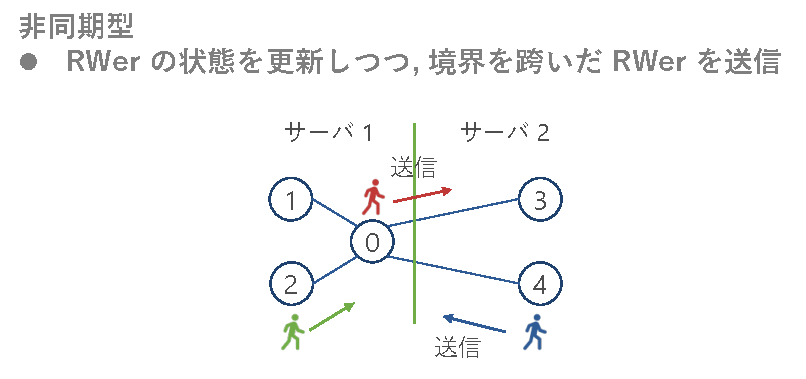
\includegraphics[scale=0.8]{figure/walkercentric_async.pdf}
    \caption{walker centric モデル (非同期型) の概要.}
    \label{walker centric モデル (非同期型) の概要}
\end{figure}

\begin{figure}[t!]
    \centering
    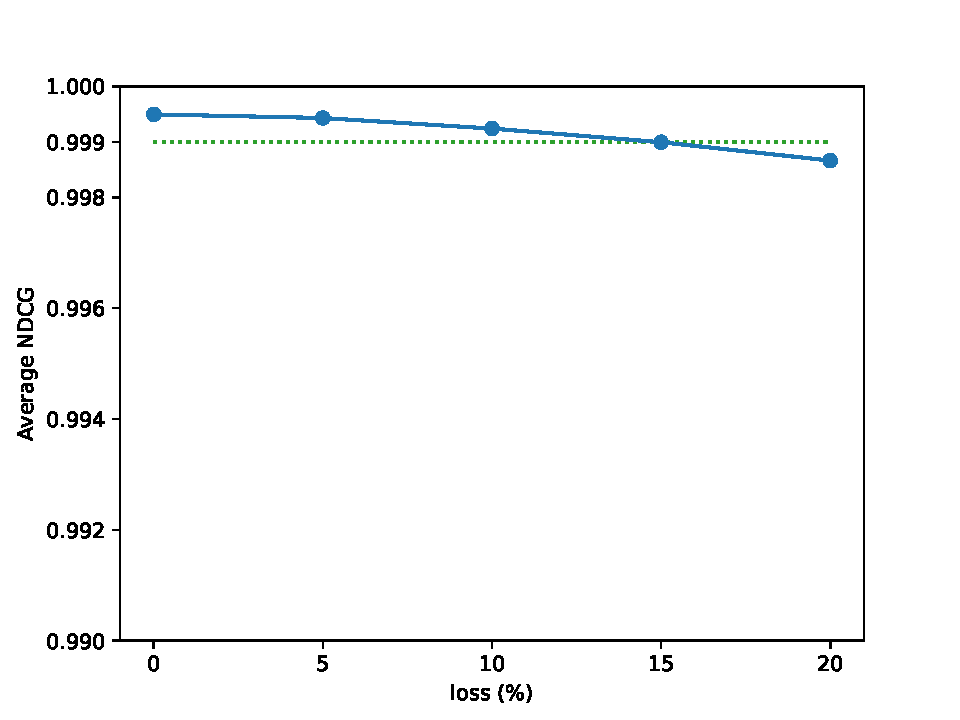
\includegraphics[scale=0.7]{figure/eva_drop.pdf}
    \caption{局所的に RWer が損失したときの PPR 演算の精度.}
    \label{局所的に RWer が損失したときの PPR 演算の精度}
\end{figure}

次に, 提案手法は RWer の送受信に UDP 通信を採用する. UDP 通信では, たとえ RTT・パケットロス率が高かったとしてもデータ転送スピードに影響しない. そのため, 地理的分散環境下における RWer の送受信には UDP 通信が適している. UDP 通信のデメリットはパケットロスが発生することであるが, RW の独立性により, RWer の損失のデメリットは少ない. 図 \ref{局所的に RWer が損失したときの PPR 演算の精度} に局所的に RWer が損失したときの Personalized PageRank (PPR) 演算の精度を示す. PPR とは, ある始点から始めた RW における各頂点の滞在確率を表している. この実験では LiveJournal のデータセット\cite{snapnets} のグラフを 5 台のサーバで分散管理し, ランダムな開始頂点から 50000 回の RW を実行することで RWer の経路情報から PPR を計算した. ここで, サーバ 1, 2, 3, 4 からサーバ 5 への RWer の送信の $x\%$ (図 \ref{局所的に RWer が損失したときの PPR 演算の精度} の横軸) を意図的に落とすことで, RWer が局所的に損失するシミュレーションを行った. PPR 演算精度を NDCG と呼ばれる指標で算出し, ランダムな開始頂点 1000 個分の平均を 図 \ref{局所的に RWer が損失したときの PPR 演算の精度} の縦軸に設定した. NDCG は 1 に近づくほど精度が高くなり, 0.999 程度あれば真値とほとんど等しい. NDCG が 0.999 を下回るのは意図的に落とす確率が 15 $\%$ のときであるため, RWer の損失が RW を利用したアプリケーションへ及ぼす影響は少ないことがわかる. 

UDP 通信の他にも QUIC と呼ばれる UDP 通信を用いて高速化しつつ TCP 通信のような通信の信頼性を提供するトランスポート層のプロトコルがある. UDP 通信に対する QUIC のメリットは, 認証・暗号化による安全性, そして再送制御による信頼性である. しかし本研究において, 安全性は現時点では不必要であり, 図 \ref{局所的に RWer が損失したときの PPR 演算の精度} のようにパケットロスの影響が少ないため再送制御も不必要である. そのため本研究では QUIC ではなく UDP 通信を採用した. 

また, 提案手法は終了した RWer の経路再利用により, RW 遷移における RWer 送受信を一部スキップする. 地理的分散環境下における RW 実行でボトルネックとなるのはサーバを跨ぐ RW 遷移による RWer の送受信である. そのため, この機能を導入することで実行時間を削減することができる. 

\section{提案手法の全体像}\label{提案手法の全体像について}

本節では提案手法の全体像について述べる. 図 \ref{提案手法の全体像} に提案手法の全体像を示す. 各サーバは独立して RWer 生成, RW 処理, 送信, 受信を自律的に行う. RW 処理では, 生成した RWer, 受信した RWer を滞在頂点からランダムに遷移させ続ける. このとき他のサーバが保持する頂点への遷移が発生した場合は, その RWer を頂点の持ち主サーバへ送信する. また, 途中で RW が終了した場合は RWer をその RWer の生成サーバへ送信する. このシステムを使用するユーザーはまず, 興味のある頂点を始点とする RWer の生成をシステムに命令し, RW 実行を開始する. その後終了して帰ってきた RWer をグラフの解析に利用することとなる. RWer の経路再利用機能では, この帰ってきた RWer の経路情報を保存しておき, 次回以降の RW 遷移に活用する. 

\begin{figure}[t]
    \centering
    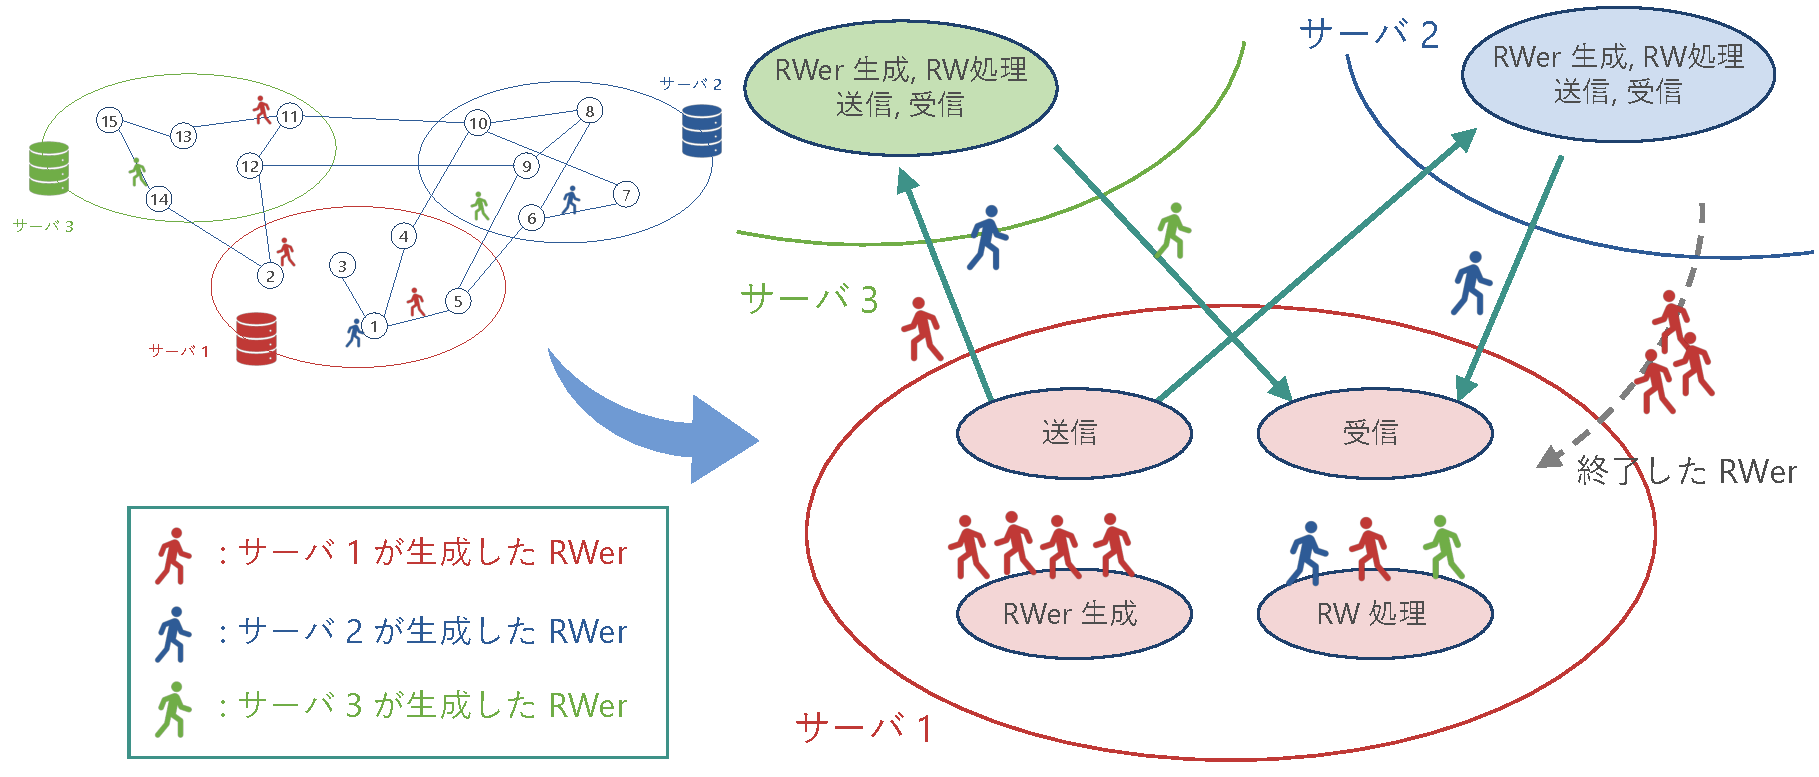
\includegraphics[scale=0.5]{figure/proposed.pdf}
    \caption{提案手法の全体像.}
    \label{提案手法の全体像}
\end{figure}

\section{Random Walker の構成}\label{Random Walker の構成}

本節では提案手法における RWer の構成について述べる. 表 \ref{RWer の構成} に RWer の構成を示す. $ver\_id\_$ はバージョンとメッセージ ID を含んでおり, メッセージ ID によって, 生存している RWer or 終了した RWer or 複数の RWer が入っているメッセージを識別する. この $ver\_id\_$ はメッセージの送受信におけるパケットにも付与するがその詳細については \ref{chap:implement} 章で述べる. $flag\_$ では RW 処理をする上で必要となる情報をフラグとして保持する. 1 hop 前で通信が発生したかを保持しておくことで, その遷移先で経路情報における通信発生フラグを立てることができる. また, $next\_index\_$ に値が入っているかを保持しておくことで, \ref{Random Walker の経路再利用} 節で説明する送信先での index による遷移を行うことができる. そして全体を通して通信が発生したかを保持しておくことで, 終了した RWer を他のサーバに送信するかどうかを判断することができる. $RWer\_size\_$ は RWer 単体のメモリサイズを保持する. これはメッセージ送信時の複数の RWer をまとめる際に必要となる. $RWer\_id\_$ は RWer の識別 ID である. $RWer\_life\_$ は RW 演算における残り hop 数を保持する. 提案手法では RWer 生成時に経路長を先に計算する. 例えば各遷移ごとで確率 $\alpha (< 1)$ で終了する RW 演算であれば, $0 < r < 1$ の乱数を $r < \alpha$ となるまで生成し, その生成回数を経路長とする. この $RWer\_life\_$ はサーバ上で RWer の構造体を生成する際, 可変長配列である $path\_$ のメモリ確保に使用される. $path\_length\_at\_current\_host\_$ は RWer の現在の同一ホスト内における経路長を保持する. これは $path\_$ における現在ホスト情報の位置を特定する際に使用される. $next\_index\_$ は通信が発生したときの次の遷移先 index を示す. これは RWer の経路再利用機能で使用される. 

\begin{table}[t]
    \caption{RWer の構成.}
    \label{RWer の構成}
    \centering
    \begin{tabular}{ccc}
        \hline \hline
        名称  &  サイズ  &  内容 \\
        \hline 
        $ver\_id\_$  &  8 bit  &  バージョン: 4 bit, メッセージ ID: 4 bit \\
        \hline
        $flag\_$  &  8 bit  & 
        \begin{tabular}{c} 1 hop 前で通信が発生したか: 1 bit, \\$next\_index\_$ に値が入っているか: 1 bit, \\全体を通して通信が発生したか: 1 bit, \\予備: 5 bit 
        \end{tabular}\\
        \hline
        $RWer\_size\_$  &  16 bit  &  RWer 単体のメモリサイズ \\
        \hline
        $RWer\_id\_$  &  32 bit  &  RWer の識別 ID \\
        \hline
        $RWer\_life\_$  &  16 bit  &  RWer の残り歩数  \\
        \hline
        $path\_length\_at\_current\_host\_$  &  16 bit  &  RWer の現在の同一ホスト内の経路長  \\
        \hline
        $reserved\_$  &  32 bit  &  予備  \\
        \hline
        $next\_index\_$  &  64 bit  &  通信が発生したときの次の遷移先 index \\
        \hline
        $path\_$  &  64 bit の可変長配列  &  経路情報  \\
        \hline
    \end{tabular}
\end{table}

\begin{figure}[t]
    \centering
    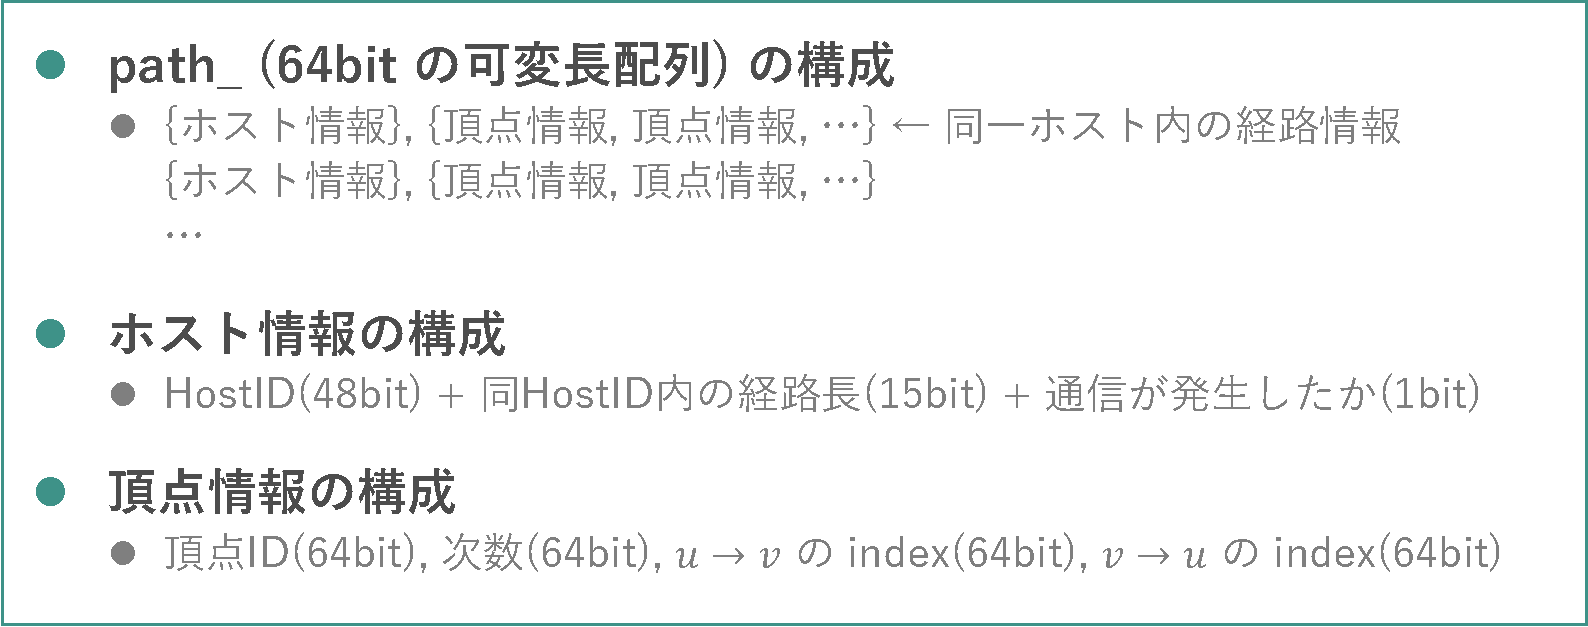
\includegraphics[scale=0.5]{figure/path.pdf}
    \caption{経路情報の構成.}
    \label{経路情報の構成}
\end{figure}

図 \ref{経路情報の構成} に $path\_$ (経路情報) の構成を示す. $path\_$ は, ホスト情報 (64 bit), 頂点情報 (64 bit $\times$ 4), 頂点情報, ... , ホスト情報, 頂点情報, ... のように頂点情報をホストごとにグループ化する. これにより各頂点情報にその頂点を保有するホストの情報を入れる必要がなくなり, サイズを削減することができる. ホスト情報の構成は, HostID (48 bit), 同一 HostID 内の経路長 (15 bit), 通信が発生したかどうかのフラグ (1 bit) である. 同一 HostID 内の経路長は経路情報を前方から探索していく際に必要となる. 通信が発生したかどうかのフラグは, 経路再利用による通信スキップが発生しなかった場合の判定に利用できる. 頂点情報の構成は, 頂点 ID (64 bit), 次数 (64 bit), $u \rightarrow v$ の index (64 bit), $v \rightarrow u$ の index (64 bit) である. $u \rightarrow v$ の index はひとつ前の頂点から見た今の頂点の index 情報であり, $v \rightarrow u$ の index は今の頂点から見たひとつ前の頂点の index 情報である. 逆方向の index 情報を保持しておくことで, 無向グラフにおける逆向きの経路情報も再利用することができる. 次数情報は経路再利用時に使用されるため頂点情報に含まれている.

\section{Random Walker の経路再利用}\label{Random Walker の経路再利用}

地理的分散環境下での RW 実行においてボトルネックとなるのは, サーバを跨ぐ RW 遷移における RWer の送受信である. 提案手法ではこの RWer の送受信を減らすため, RWer の経路再利用による通信スキップ機能を追加する. 図 \ref{RWer の経路再利用機能の概要} に RWer の経路再利用機能の概要を示す. 図の左上では, サーバ 1 上の頂点 1 を始点とする RW がサーバ 3 上の頂点 13 で終了した状態を表しており, その後サーバ 3 は終了した RWer を生成サーバであるサーバ 1 へ送信する. 生成サーバであるサーバ 1 は自身が所有するグラフとその周辺の解析のためにこの終了した RWer を利用するため, サーバ 3 からサーバ 1 への RWer 送信は RWer の経路再利用のためだけに追加した処理ではない. 図の右下は, サーバ 1 がサーバ 3 から RWer を受信した後での, サーバ 1 上の頂点 4 からサーバ 2 上の頂点 10 への RW 遷移を表している. 通常, 所有サーバが異なる頂点間の遷移では RWer の送受信が発生するが, 以前に受信した RWer の経路情報の一部 (頂点 10 の次数や index 情報) を利用することによって, サーバ 1 からサーバ 2 への送信をスキップすることができる. 本手法における RW 遷移の一般的な手順は Algorithm \ref{RW 遷移} に示す.

\begin{figure}[t]
    \centering
    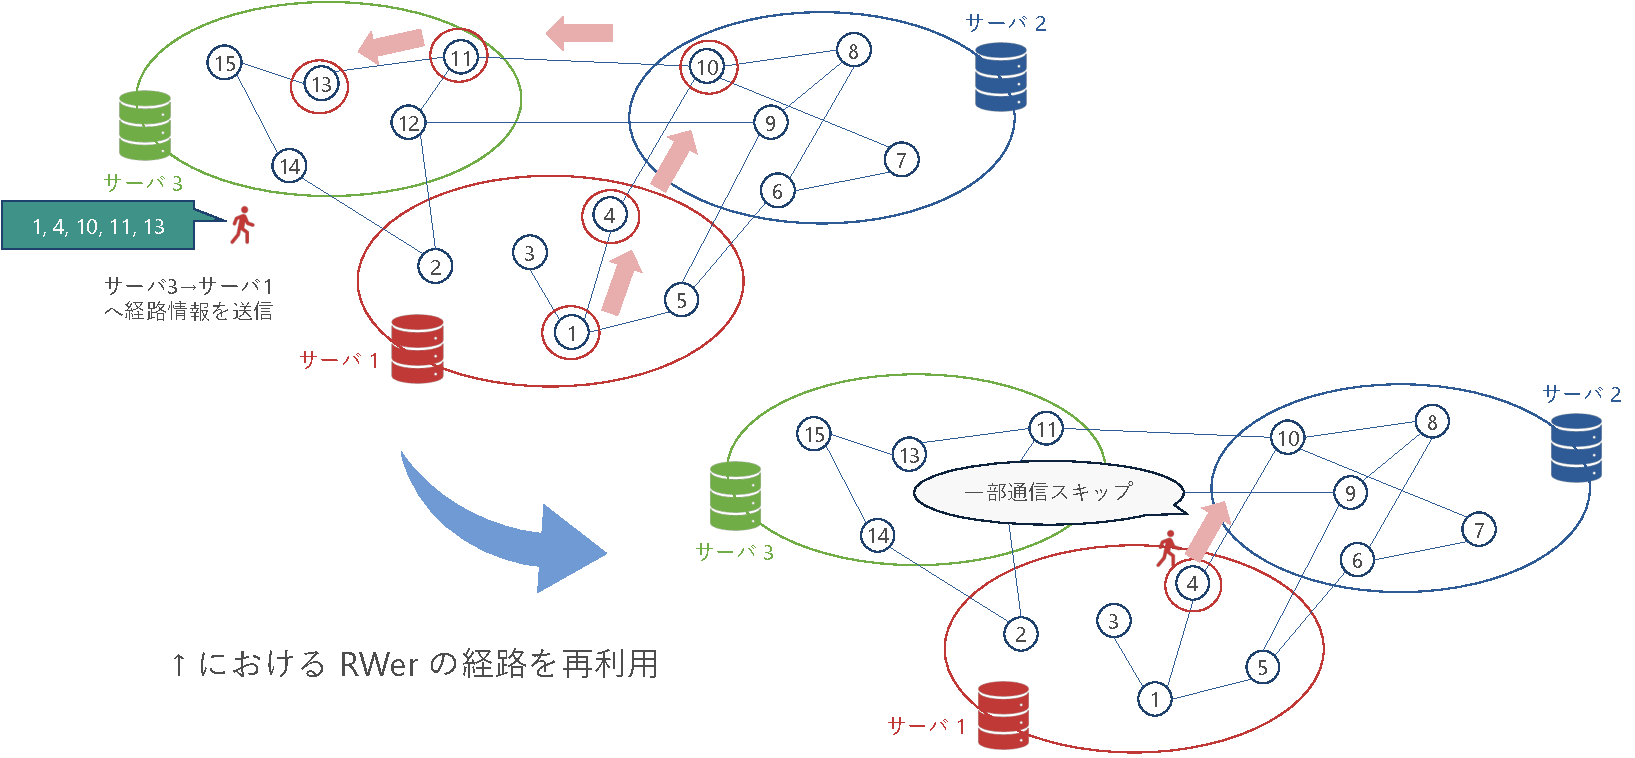
\includegraphics[scale=0.5]{figure/cache_gai.pdf}
    \caption{RWer の経路再利用機能の概要.}
    \label{RWer の経路再利用機能の概要}
\end{figure}

\begin{algorithm}[t]
\DontPrintSemicolon
\nl     $v \leftarrow$ RWer が滞在している頂点\;
\nl     \If{$v$ が自サーバの所有頂点である} {
\nl         \If{RWer に次の遷移先の index 情報が格納されている} {
\nl             その情報通りに RWer を遷移させる\;}
\nl         \Else {
\nl             ランダムに遷移\;}}
\nl     \ElseIf{$v$ が自サーバの所有頂点でない} {
\nl         $degree \leftarrow$ 過去の経路情報から得られた $v$ の次数\;
\nl         $next\_index \leftarrow 0 \leq r < degree$ のランダムな値\;
\nl         $next\_node \leftarrow v$ の $next\_index$ 番目の隣接頂点\;
\nl         \If{$next\_node$ が過去の経路情報から得られなかった場合} {
\nl             $RWer$ に $next\_index$ の情報を格納し, $v$ の持ち主サーバへ送信\;}
\nl         \Else {
\nl             $RWer$ を $next\_node$ に遷移させる (通信スキップ)\;}}
\caption{{RW 遷移} \label{RW 遷移}}
\end{algorithm}

図 \ref{具体例における RWer の経路情報} は図 \ref{RWer の経路再利用機能の概要} の RWer の経路情報を具体的に示したものである. 頂点の周りに記載されている数字は index 情報を示している. 例えば頂点 1 から見た頂点 4 の index は 1 となる. この index 情報は頂点 ID の昇順で各頂点に振り分けられる. サーバ 3 での RW 終了時, RWer はサーバ 1 へ送信されるため, サーバ 1 がこの経路情報を保有する. 図 \ref{経路再利用による送信スキップ} に経路再利用による送信スキップの詳細を示す. サーバ 1 上で頂点 4 から頂点 10 への遷移が決まった後, サーバ 1 は経路情報から頂点 10 の次数が 4 であることを知っているため, 頂点 10 の次の遷移先 index をランダムに選択する. 遷移先 index が 0, 3 の場合は経路情報からそれぞれ頂点 4, 頂点 11 へ遷移することがわかるため, サーバ 1 上で遷移を行う. 遷移先 index が 1, 2 の場合は経路情報から遷移先がわからないため, サーバ 2 へ送信することになる. このとき, 表 \ref{RWer の構成} の $next\_index\_$ に index 情報を格納する. そしてサーバ 2 が RWer 受信したのち, この index 情報を利用して RW の遷移を行う. この例では頂点 4 から頂点 10 への遷移におけるサーバ間の RWer 送信が 4 分の 2 の確率でスキップされることになる. サーバ 1 上で頂点 10 から頂点 11 への遷移が決まった場合は, 頂点 11 からの遷移に関しても頂点 10 と同様にしてその先の遷移を行うことができる. 

\begin{figure}[t]
    \centering
    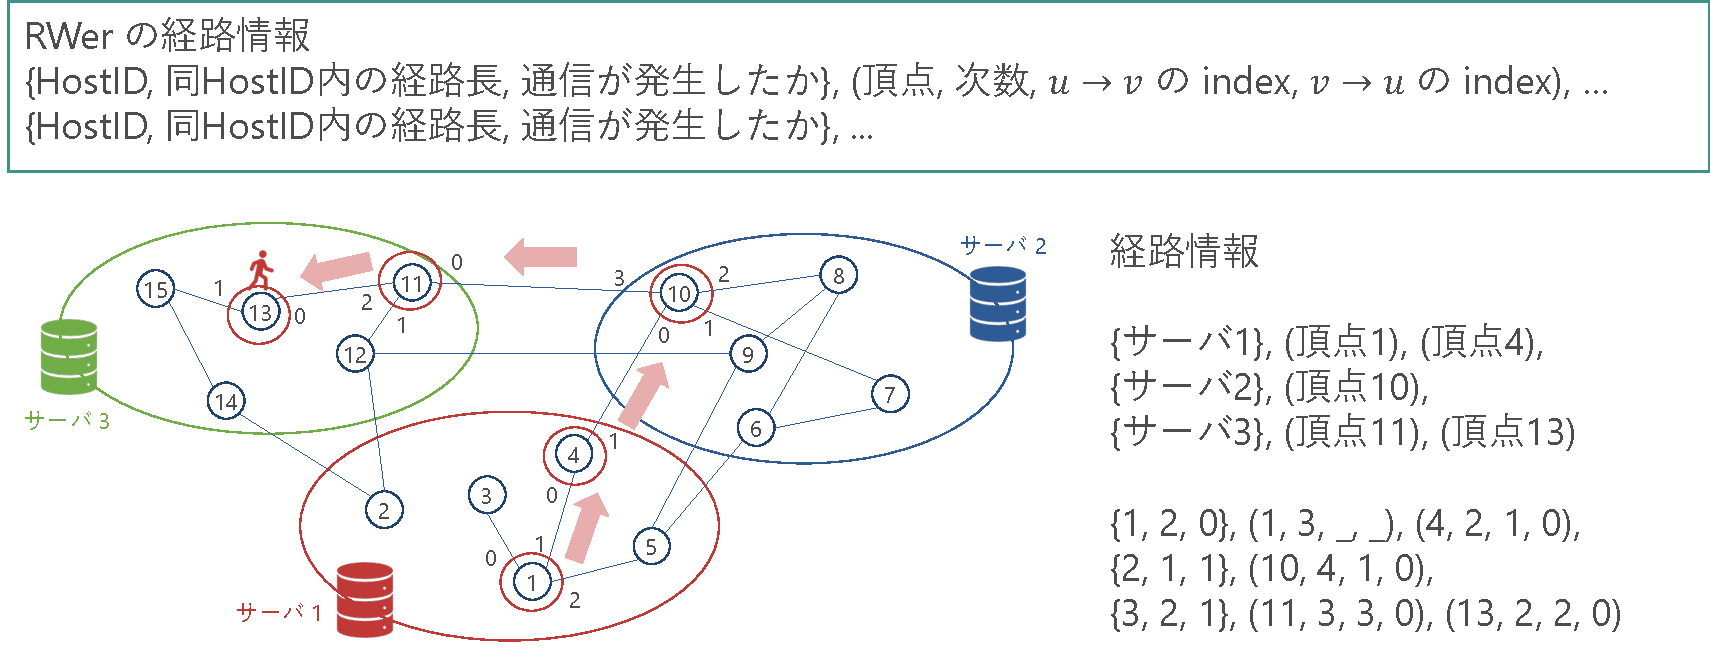
\includegraphics[scale=0.5]{figure/path_ex.pdf}
    \caption{具体例における RWer の経路情報.}
    \label{具体例における RWer の経路情報}
\end{figure}

\begin{figure}[t]
    \centering
    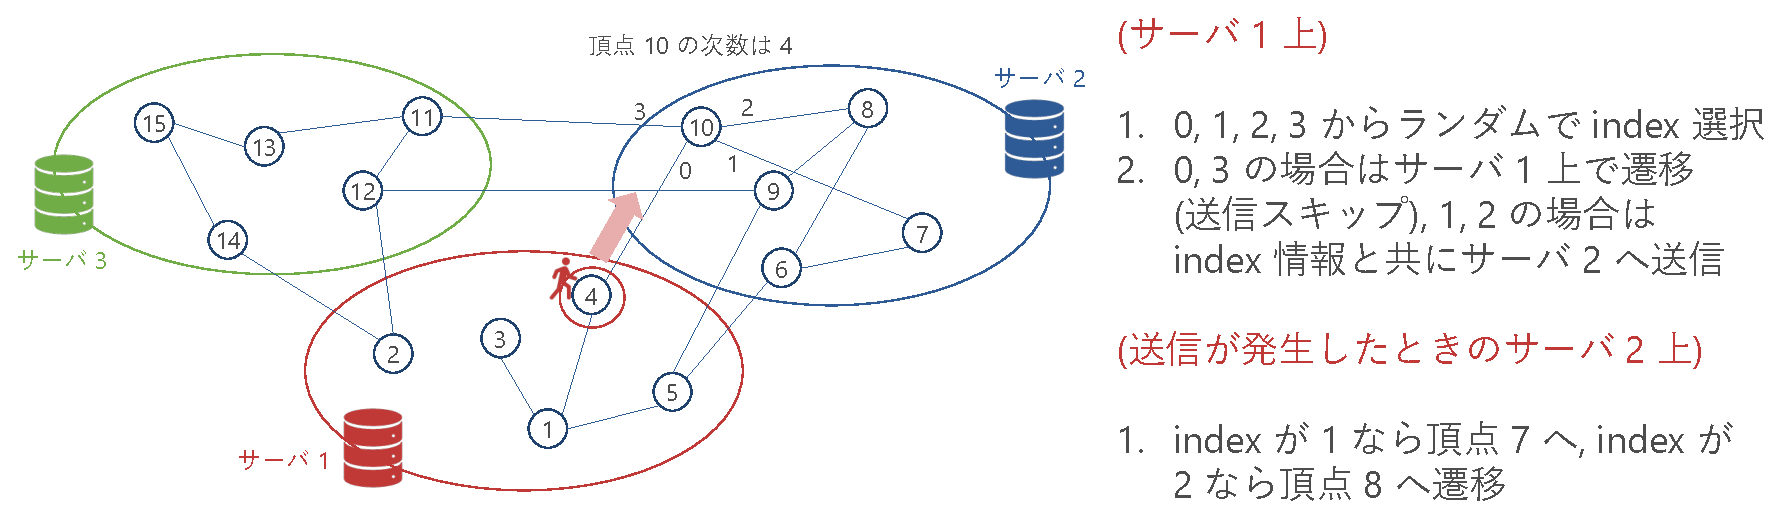
\includegraphics[scale=0.5]{figure/skip.pdf}
    \caption{経路再利用による送信スキップ.}
    \label{経路再利用による送信スキップ}
\end{figure}

% \section{実装}\label{実装}

% 本節では提案手法の実装について述べる. 図 \ref{サーバ上の実装の概要} に実装の概要を示す. 提案手法はサーバクラスタによる分散グラフ処理システムであるため, 各サーバ上でこの実装によるプログラムが動作する. RWer 生成 \& 処理スレッドでは, RWer を生成しその後 RW 処理を行う. このとき他のサーバが所有する頂点への遷移が発生した場合は, その RWer を送信キューに格納する. 受信スレッドでは, 他のサーバからメッセージを受信し, そのメッセージの種類に応じた処理を行う. 例えばメッセージが複数の RWer を含むものだった場合は, それらの RWer を RWer キューに格納する. RWer 処理スレッドでは, RWer キューから RWer をまとめて取り出し, RW 処理を行い, 他のサーバが所有する頂点への遷移が発生した場合は, その RWer を送信キューに格納する. 送信スレッドでは, 送信先ごとの送信キューから RWer をまとめて取り出し, 他のサーバへ送信する. 以降, 終了した Random Walker の経路情報の保持方法, 受信スレッド, RWer 処理スレッド, 送信スレッドの 4 つについて, 適宜擬似コードを用いて詳細を説明する. 

% \begin{figure}[t]
%     \centering
%     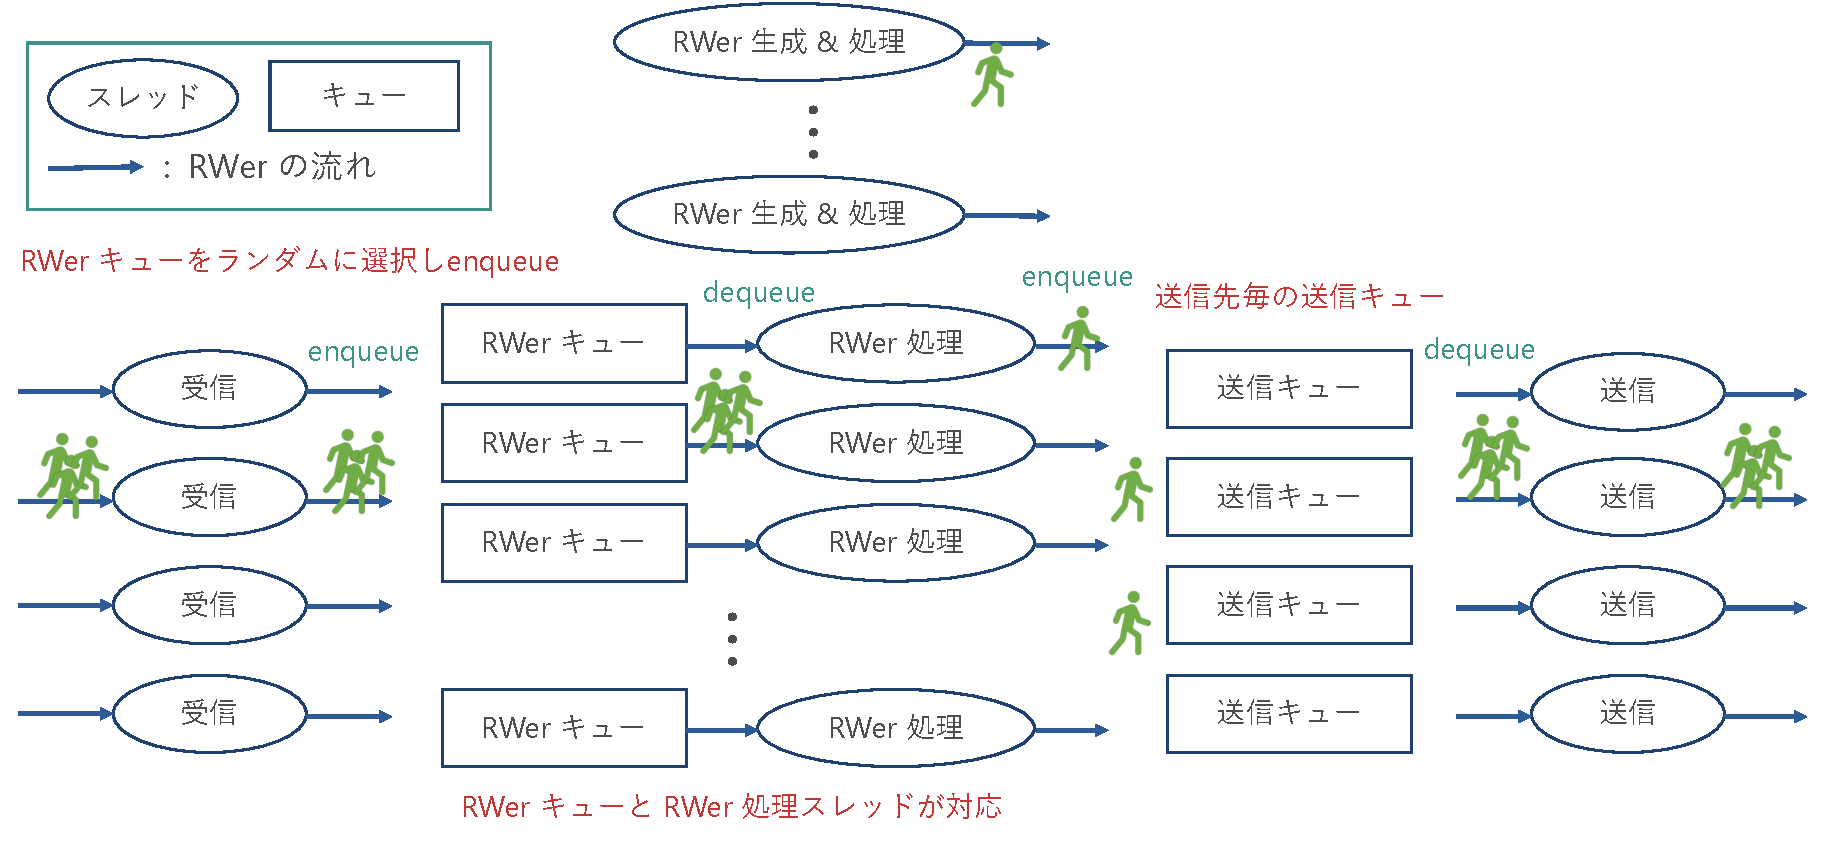
\includegraphics[scale=0.5]{figure/implementation.pdf}
%     \caption{サーバ上の実装の概要}
%     \label{サーバ上の実装の概要}
% \end{figure}

% \subsection{終了した Random Walker の経路情報の保持方法}

% \ref{Random Walker の経路再利用} で説明したように, 本手法では終了した RWer の経路情報を再利用することで通信のスキップを行う. そのためには終了した RWer の経路情報を保存しておく必要がある. 経路情報のまま保存するのは無駄が多いため, 経路再利用時に必要となる項目ごとに情報を保存する. 表 \ref{Random Walker の経路情報の保存形式} に RWer の経路情報の保存形式を示す. 本手法は C++ を使って実装しているためデータ構造は C++ の形式で記述した. 頂点に対する次数は RW 遷移時における index 選択の際に必要となる. データ構造に関しては, 頂点 ID を index とした配列の形で保持する. 頂点に対する持ち主サーバは, もし次の遷移先情報を持っていない場合に現在頂点の持ち主サーバへの RWer の送信が発生するため, 必要である. データ構造に関しては次数情報と同様, 頂点 ID を index とした配列の形で保持する. エッジデータは index を使った RW 遷移に必要となる. 例えば図 \ref{経路再利用による送信スキップ} ではサーバ 1 が (10, 0, 4), (10, 3, 11) (始点頂点, index, 遷移先頂点) というエッジデータを保持しているため, index = 0, 3 の場合は通信をスキップすることができる. データ構造に関しては, 頂点 ID を index とし, それぞれの頂点について (key, value) = (index, 遷移先頂点) のハッシュ map を保持する形とした. 

% \begin{table}[t]
%     \caption{Random Walker の経路情報の保存形式}
%     \label{Random Walker の経路情報の保存形式}
%     \centering
%     \begin{tabular}{cc}
%         \hline
%         保存項目  &  データ構造 (C++)  \\
%         \hline \hline
%         頂点に対する次数  &  std::vector$\langle$uint64$\_$t$\rangle$ \\
%         \hline
%         頂点に対する持ち主サーバ  &  std::vector$\langle$uint64$\_$t$\rangle$  \\
%         \hline
%         エッジデータ  &  std::vector$\langle$std::unordered$\_$map$\langle$uint64$\_$t, uint64$\_$t$\rangle$$\rangle$ \\
%         \hline
%     \end{tabular}
% \end{table}

% \subsection{受信スレッド}

% \begin{algorithm}[t]
% \DontPrintSemicolon
% \nl $message \leftarrow$ 受信データ\;
% \nl $message\_id \leftarrow message$ の先頭から抜き出した値\;
% \nl \If{$message\_id ==$ 複数の RWer によるメッセージ} {
% \nl     $RWer\_count \leftarrow message$ の先頭から抜き出した値\;
% \nl     $RWer \;\; A[RWer\_count]$\;
% \nl     $idx \leftarrow message$ 内における先頭の RWer 情報の開始位置\;
% \nl     \For{$i = 1$ to $RWer\_count$} {
% \nl         $A[i] \leftarrow message 内における i$ 個目の RWer の情報\;
% \nl         $idx \leftarrow idx$ + ($i$ 個目の RWer のメモリサイズ)\;}
% \nl     RWer キューをランダムに選択し, $A$ 内の RWer を全て格納\;}
% \nl \Else{
% \nl     他の場合は説明省略\;}
% \caption{{受信スレッド} \label{受信スレッド}}
% \end{algorithm}

% \begin{table}[t!]
%     \caption{メッセージの構成}
%     \label{メッセージの構成}
%     \centering
%     \begin{tabular}{ccc}
%         \hline
%         名称  &  サイズ  &  内容 \\
%         \hline \hline
%         $ver\_id\_$  &  8 bit  &  バージョン: 4 bit, メッセージ ID: 4 bit \\
%         \hline
%         $RWer\_count$  &  16 bit  &  メッセージ内に含まれる RWer の数 \\
%         \hline
%         複数の RWer  &  可変長サイズ $\times$ $RWer\_count$  &  表 \ref{RWer の構成} の RWer の情報を複数格納 \\
%         \hline
%     \end{tabular}
% \end{table}

% 受信スレッドでは, 他のサーバから受信したメッセージを処理し, 適宜 RWer を RWer キューに格納する. メッセージの種類は複数の RWer 以外にも実験開始の合図, 結果送信の合図等があるが, ここでは主要な処理である複数の RWer について説明する. Algorithm \ref{受信スレッド} に受信スレッドの擬似コードを示す. また, 提案手法におけるメッセージ構成を表 \ref{メッセージの構成} に示す. まず, 受信したメッセージを $message$ に格納し, $message\_id$ を先頭の $ver\_id\_$ から抽出する (1, 2 行目). 次に $message$ からメッセージ内の RWer の個数である $RWer\_count$ を抽出し, サイズ $RWer\_count$ の RWer 格納用配列を作成する (4, 5 行目). そしてその配列 $A$ に $message$ 内の RWer の情報を格納していく(6 -- 9 行目). $idx$ は $message$ 内におけるそれぞれの RWer の情報の開始位置を表す. つまり, 6 行目において $idx$ = 24 bit であり, RWer の情報の開始位置は先頭から 25 bit 目である. RWer の情報は可変長なので, 2 つ目以降の RWer に関する $idx$ については, その都度一つ前の RWer のメモリサイズを表 \ref{RWer の構成} の $RWer\_size$ から読み取り, 加算する(9 行目). 最後に, 格納先の RWer キューをランダムに一つ選択し, $A$ 内の RWer を全て格納する(10 行目). 本手法では, 並列性を可能な限り保つことができる構築を意識しており, 受信スレッドごとに異なるポート番号を振り分け, 受信処理を並列に行う. また, RWer 処理スレッドも同様で, 図 \ref{サーバ上の実装の概要} のように各 RWer スレッドごとに RWer キューを用意した. 10 行目における RWer キューのランダム選択は, 各 RWer 処理スレッドの負荷分散のためである. また, $A$ 内の RWer それぞれに対してランダムな RWer キューを選択するのではなく, $A$ 内の全ての RWer をまとめて一つの RWer キューに格納するのは, RWer キューにて必要となる排他制御のロックを低減させるためである. 

% 本手法ではスレッド間での情報のやり取りが多い. 例えば, 受信スレッドと RWer 処理スレッド間では RWer キューを通じて RWer を受け渡す. ここでもし RWer を構造体のまま RWer キューへ push, または RWer キューから pull しようとすると, その都度構造体のメモリコピーが発生してしまいオーバヘッドが大きくなる. そのため本手法では情報の受け渡しをポインタで行う. また, スレッド間でのポインタの受け渡しには所有権の概念が存在するため, C++ におけるスマートポインタを利用してこの処理を実装した. 



% \subsection{RWer 処理スレッド}

% RWer 処理スレッドでは, RWer キューから RWer をまとめて取り出し, それぞれの RWer に対して RW 処理を行い, 他のサーバが所有する頂点への遷移が発生した場合は, その RWer を送信キューに格納する. Algorithm \ref{RWer 処理スレッド} に RWer 処理スレッドの擬似コードを示す. まず RWer キューから RWer をまとめて取り出し, 配列 $A$ に格納する(1, 2 行目). そして $A$ 内の各 $RWer$ について RW 処理を行う(3 -- 38 行目). RW 処理については, まず $RWer$ の $ver\_id\_$ (表 \ref{RWer の構成} 参照) から $message\_id$ を抽出し, それがもし終了した RWer のものだった場合, 終了した RWer に対する処理を行う(4 -- 6 行目). 終了した RWer に対する処理では主にその RWer の生成サーバに対応する送信キューへの push を行う. $message\_id$ が, まだ生存している RWer のものであった場合は, その RWer が終了 or 他のサーバが所有する頂点へ遷移し, 送信キューに格納されるまで処理を繰り返し行う(7 -- 38 行目). ここでの処理は $RWer$ の現在頂点である $current\_node$ (9 行目)が自サーバの所有頂点である場合とそうでない場合で異なる. $current\_node$ が自サーバの所有頂点である場合は, 基本的には自分が所持するグラフ上でのランダム遷移を行う. しかし 1 hop 前で通信が発生した, かつ $RWer$ の $next\_index\_$ (表 \ref{RWer の構成} 参照) に index 情報が格納されている場合は, 次の遷移はその index 情報を利用して行う(11 -- 14 行目). これは図 \ref{経路再利用による送信スキップ} の送信が発生したときのサーバ 2 上での処理に対応している. 遷移先 index のランダム選択は送信前に済ませているため, 送信先で再びランダム選択を行うと不正確な RW 遷移となってしまう. $current\_node$ が自サーバの所有頂点でない場合は, 過去の RWer の経路情報を利用して RW 遷移を行う. 22 行目における, 過去の経路情報から $current\_node$ の次数がわからない場合は, $current\_node$ が, 自分が所有する頂点の隣接頂点のうち, 他サーバが所有するかつまだ経路情報に含まれていない頂点であることがわかる. 本手法が想定する分散グラフ管理下では, 隣接頂点が他サーバの所有する頂点である場合, 自サーバはその頂点の ID と持ち主サーバの情報のみを保持するとしているため, $current\_node$ が自サーバの所有頂点でない (他サーバの頂点 ID 情報を持っている) かつ $current\_node$ の次数情報を持っていないという状態が存在する場合がある. このときは, $RWer$ を $current\_node$ の持ち主サーバへの送信キューへ push する(22, 23 行目). ここでは次数がわからず, index のランダム選択は行わない($RWer$ の $next\_index\_$ に値を入れない)ため, この $RWer$ を受信したサーバは, 11 行目における if 文を通過し, 通常のランダム遷移を行う. $current\_node$ の次数 ($degree$) が過去の経路情報からわかる場合, $degree$ 未満のランダムな値を $next\_index$ として, $current\_node$ の $next\_index$ 番目の隣接頂点を次の遷移先頂点 ($next\_node$) とする(26, 31, 32 行目). ここで, $next\_node$ が過去の経路情報から得られなかった場合は, $RWer$ の $next\_index\_$ に $next\_index$ を入れ, $current\_node$ の持ち主サーバへの送信キューへ push する(33 -- 35 行目). これは図 \ref{経路再利用による送信スキップ} において, サーバ 1 上で 1 or 2 の index を選択した場合に対応する. この RWer を受信したサーバは, 11 行目の if 分で引っかかり, index 情報による決定的な遷移を行う. $next\_node$ が過去の経路情報から得られた場合は, $RWer$ をその $next\_node$ に遷移させる(38 行目). 
% \\
% \\
% \\
% \\

% \begin{algorithm}[p]
% \DontPrintSemicolon
% \nl vector$\langle$RWer$\rangle$ $\; A$\;
% \nl $A \leftarrow$ RWer キューから RWer をまとめて取り出し, 格納\;
% \nl \For{$each \; RWer \in A$} {
% \nl     $message\_id \leftarrow RWer$ の $ver\_id\_$ から抽出\;
% \nl     \If{$message\_id ==$ 終了した RWer} {
% \nl         終了した RWer に対する処理\;}
% \nl     \ElseIf{$message\_id ==$ 生存している RWer} {
% \nl         \While{true} {
% \nl             $current\_node \leftarrow RWer$ の現在頂点\;
% \nl             \If{$current\_node$ が自サーバの所有頂点である場合} {
% \nl                 \If{1 hop 前で通信が発生した $\&\&$ 次の遷移先の index 情報が格納されている} {
% \nl                     $next\_index \leftarrow RWer の next\_index\_$\;
% \nl                     $next\_node \leftarrow$ $current\_node$ の隣接リストの $next\_index$ 番目の頂点\;
% \nl                     $RWer$ を $next\_node$ に遷移させる\;}
% \nl                 \ElseIf{$RWer$ の $RWer\_life\_$ が 0 \textbar\textbar $\;current\_node$ の次数が 0} {
% \nl                     終了した RWer に対する処理\;
% \nl                     break\;}
% \nl                 \Else {
% \nl                     $next\_node \leftarrow$ $current\_node$ のランダムな隣接頂点\;
% \nl                     $RWer$ を $next\_node$ に遷移させる\;}}
% \nl             \ElseIf{$current\_node$ が自サーバの所有頂点でない場合} {
% \nl                 \If{過去の経路情報から $current\_node$ の次数情報がわからない場合} {
% \nl                     $current\_node$ の持ち主サーバへの送信キューに $RWer$ を push\;
% \nl                     break\;}
% \nl                 \Else {
% \nl                     $degree \leftarrow$ 過去の経路情報から得られた $current\_node$ の次数\;
% \nl                     \If{$RWer$ の $RWer\_life\_$ が 0 \textbar\textbar $\;degree == 0$} {
% \nl                         終了した RWer に対する処理\;
% \nl                         break\;}
% \nl                     \Else {
% \nl                         $next\_index \leftarrow 0 \leq r < degree$ のランダムな値 $r$\;
% \nl                         $next\_node \leftarrow current\_node$ の $next\_index$ 番目の隣接頂点\;
% \nl                         \If{$next\_node$ が過去の経路情報から得られなかった場合} {
% \nl                             $RWer$ の $next\_index\_ \leftarrow next\_index$\;
% \nl                             $current\_node$ の持ち主サーバへの送信キューに $RWer$ を push\;
% \nl                             break\;}
% \nl                         \Else {
% \nl                             $RWer$ を $next\_node$ に遷移させる\;}}}}}}}
% \caption{{RWer 処理スレッド} \label{RWer 処理スレッド}}
% \end{algorithm}

% \subsection{送信スレッド}\label{sub:送信スレッド}

% 送信スレッドでは, 送信先ごとの送信キューから RWer をまとめて取り出し, メッセージを生成し,他サーバへ送信する. Algorithm \ref{送信スレッド} に送信スレッドの擬似コードを示す. 1 -- 3 行目は各送信スレッドがどの送信キューを選択するかを決める処理を表している. 本手法では送信キューが送信先ごとに生成されるのに対し送信スレッド数は最初から決まっているため, それぞれの送信スレッドはどの送信キューに格納されている RWer を送信するのかを決める必要がある. 送信スレッド間で同時に同じ送信キューが選択されることを防ぐため, 1 -- 3 行目は送信スレッド間での排他制御となっている. $id\_num\_$ は全送信スレッド間での共有変数であり, 暫定送信先 ID を示す. この $id\_num\_$ が自サーバのものでないかつ, 他のサーバが $id\_num\_$ 番目の送信キューを占有していない状態を満たすまで $id\_num\_$ をインクリメントする(1 -- 2 行目). 条件を満たす $id\_num\_$ が得られたらスレッド内変数である $send\_id$ に格納する(3 行目). その後, $send\_id$ 番目の送信キューから RWer をまとめて取り出し, 配列 $A$ に格納する. 6 行目以降は配列 $A$ 内の $RWer$ をできるだけまとめながら送信する処理を表している. $message$ は送信するメッセージを入れる変数, $RWer\_count$ は一つのメッセージ内に含まれる RWer の数, $now\_message\_size$ は現在のメッセージサイズを示しており(6 -- 8 行目), メッセージサイズの初期値は $ver\_id\_$ と $RWer\_count$ のサイズの合計である 24 となる (表 \ref{メッセージの構成}). 9 -- 20 行目の for 文ではメッセージに $RWer$ のデータを書き込んでいくが, その際メッセージサイズが指定された最大サイズを超えてしまう場合はデータ書き込みの前にメッセージ送信を行う. 送信時のポート番号については受信ポート番号からランダムに一つ選択し, 設定する. メッセージ送信後は $message$, $RWer\_count$, $now\_message\_size$ を初期値に戻す. 全ての $RWer$ のメッセージへの書き込みが終わった後, メッセージ内に $RWer$ が残っていた場合はその $message$ を送信する(21, 22 行目). 送信におけるメッセージの最大サイズについては, MTU - IP ヘッダ (20 byte) - UDP ヘッダ (8 byte) とする. 送信データサイズが MTU を超えるとパケット分割が発生し, パケットロス時の RWer 損失数が増えてしまうためである. 実験においては MTU を 9000 に設定しているため, 送信スレッドにおけるメッセージの最大サイズは 8972 byte となる. 

% \begin{algorithm}[t!]
% \DontPrintSemicolon
% \nl \While{$id\_num\_ == hostid\_ \;$ \textbar\textbar 他のサーバが $id\_num\_$ 番目の送信キューを占有している} {
% \nl     $id\_num\_ \leftarrow (id\_num\_ + 1)\; \%$ 送信キューの数\;}
% \nl $send\_id \leftarrow id\_num\_$\;
% \nl vector$\langle$RWer$\rangle$ $\; A$\;
% \nl $A \leftarrow send\_id$ 番目の送信キューから RWer をまとめて取り出し, 格納\;
% \nl $message \leftarrow$ 空のメッセージ\;
% \nl $RWer\_count \leftarrow 0$\;
% \nl $now\_message\_size \leftarrow $ sizeof($ver\_id\_$) + sizeof($RWer\_count$)\;
% \nl \For{$each \; RWer \in A$} {
% \nl     $RWer\_size \leftarrow RWer$ のメモリサイズ\;
% \nl     \If{$now\_message\_size + RWer\_size \geq $ メッセージの最大サイズ} {
% \nl         $message$ に $ver\_id\_$ と $RWer\_count$ を格納\;
% \nl         $port\_num \leftarrow$ 指定されたポート番号の中からランダム選択\;
% \nl         $message$ を $send\_id$ の送信先へ送信 (ポート番号は $port\_num$)\;
% \nl         $message \leftarrow$ 空のメッセージ\;
% \nl         $RWer\_count \leftarrow 0$\;
% \nl         $now\_message\_size \leftarrow $ sizeof($ver\_id\_$) + sizeof($RWer\_count$)\;}
% \nl     $RWer$ を $message$ に書き込む\;
% \nl     $RWer\_count \leftarrow RWer\_count + 1$\;
% \nl     $now\_message\_size \leftarrow now\_message\_size + RWer\_size$\;}
% \nl \If{$RWer\_count > 0$} {
% \nl     残った $message$ を上記と同様にして送信\;}
% \caption{{送信スレッド} \label{送信スレッド}}
% \end{algorithm}